\documentclass[12pt,a4paper]{article}

\usepackage{a4wide}
\usepackage{graphicx}
\usepackage{amsmath}
\usepackage{ae,aecompl}
\usepackage{amsthm}

%\pagestyle{empty}
\setlength{\parindent}{0pt}
\renewcommand{\labelenumi}{\alph{enumi})}
\renewcommand{\labelenumii}{\roman{enumii})}

% Neutrino oscillation channels
\newcommand{\ee}{\ensuremath{\nu_e \rightarrow \nu_e}}
\newcommand{\emu}{\ensuremath{\nu_e \rightarrow \nu_\mu}}
\newcommand{\etau}{\ensuremath{\nu_e \rightarrow \nu_\tau}}
\newcommand{\mue}{\ensuremath{\nu_\mu \rightarrow \nu_e}}
\newcommand{\mumu}{\ensuremath{\nu_\mu \rightarrow \nu_\mu}}
\newcommand{\mutau}{\ensuremath{\nu_\mu \rightarrow \nu_\tau}}
\newcommand{\taue}{\ensuremath{\nu_\tau \rightarrow \nu_e}}
\newcommand{\taumu}{\ensuremath{\nu_\tau \rightarrow \nu_\mu}}
\newcommand{\tautau}{\ensuremath{\nu_\tau \rightarrow \nu_\tau}}

% Neutrino oscillation parameters
\newcommand{\sthsol}{\ensuremath{\sin^2 2\theta_{12}}}     % Mixing angles
\newcommand{\sthchooz}{\ensuremath{\sin^2 2\theta_{13}}}
\newcommand{\sthatm}{\ensuremath{\sin^2 2\theta_{23}}}
\newcommand{\sthtf}{\ensuremath{\sin^2 2\theta_{2f}}}
\newcommand{\ldm}{\ensuremath{{\Delta m_{31}^2}}}          % Mass squared differences
\newcommand{\sdm}{\ensuremath{{\Delta m_{21}^2}}}

% Important neutrino experiments
\newcommand{\TtoK}{{\sffamily T2K}}

% Miscellaneous commands
\newcommand{\aufg}[2]{\vspace{4mm}{\bf\underline{Problem #1:} {#2}} \vspace{3mm}}

% Environment for API reference entries
\newtheoremstyle{dotless}{}{}{\itshape}{}{\bfseries}{}{0cm}{}
\theoremstyle{dotless}
\newtheorem*{function}{}

\begin{document}
\vspace*{-3cm}
\begin{center}
{\large\bf GLoBES Tutorial: Simulating accelerator neutrino experiments}\\[0.3cm]
GLoBES workshop in Heidelberg, Germany, January 24-26, 2007
\end{center}
\vspace*{2mm}

Joachim Kopp \hfill 25.01.07

\bigskip
\hrule
\vspace*{4mm}

{\small
This tutorial will introduce some of the basic concepts required to simulate
accelerator neutrino experiments with GLoBES (General Long Baseline Experiment
Simulator). We will start from a simple and incomplete implementation of the
\TtoK\ superbeam experiment, which we will gradually improve. We will first consider
the precision measurement of the leading atmospheric oscillation parameters
$\theta_{23}$ and $\ldm$, and later discuss the possible detection of
non-zero $\theta_{13}$ and $\delta_{CP}$.
}


% ----------------------------------------------------------------------------
\section*{Part 1: Precision measurement of $\theta_{23}$ and $\ldm$}
% ----------------------------------------------------------------------------

\aufg{1}{Warm-up}

Consider first the program in the directory {\tt globes-tutorials/th23dm31/},
which computes $\chi^2$ as a function of the fit values of $\theta_{23}$
and $\ldm$, but is still lacking several important features. Compile
the program by typing {\tt make} and run it with the command {\tt ./th23dm31}.
Each line of the output file {\tt th23dm31.dat} will contain three numbers:
the fit value for $\theta_{23}$ in degrees, the fit value for $\ldm$ in eV$^2$,
and the corresponding $\chi^2$. Use the script {\tt th23dm31.gnuplot}
to view the results as an EPS plot, which should look like
Fig.~\ref{fig:th23dm31-orig}.

Now, familiarize yourself with the C code ({\tt th23dm31.c}) and the AEDL
experiment definition ({\tt T2K-tutorial.glb}). In doing so, you
can already watch out for the aforementioned shortcomings of the code.
There are essentially three of them, which we will one by one discuss
below in problems 2, 4, and 5.

\begin{figure}
  \begin{center}
    \includegraphics{T2K-1}
  \end{center}
  \vspace{-0.7 cm}
  \caption{Output of {\tt th23dm31}: Confidence regions in the $\theta_{23}$--$\ldm$
    plane for a (too) simple implementation of the \TtoK\ experiment.}
  \label{fig:th23dm31-orig}
\end{figure}


\aufg{2}{Spectral analysis vs.\ total rates}

Let us examine Fig.~\ref{fig:th23dm31-orig} more closely: There is
a very strong correlation between $\theta_{23}$ and $\ldm$: A mixing angle
far from its assumed ``true'' value of $45^\circ$ is still compatible with the
data, if, at the same time, a larger $\ldm$ is assumed. The reason for this
is, that increasing $\ldm$ means that larger parts of the neutrino energy
spectrum are affected by oscillations, which compensates the smaller
oscillation amplitude. This woul be a severe limitation to the sensitivity
of the experiments, but luckily, it can be remedied by an improved data
analysis: Instead of performing a total rates analysis, we should incorporate
spectral information. Then, we can determine the energy at which the first
oscillation maximum occurs, and thus pin down $\ldm$.

Accordingly, we have to increase the number of analysis bins ({\tt \$bins}) from {\tt 1}
to {\tt 20} and select a different $\chi^2$ function in {\tt T2K-tutorial.glb}.
Change the command {\tt @sys\_on\_function = "chiTotalRatesTilt"} to
{\tt @sys\_on\_function = "chiSpectrumTilt"} in the first two rules
({\tt \#NU\_E\_Appearance\_QE} and {\tt \#NU\_MU\_Disappearance\_QE}).
Leave the charged current $\nu_e$ appearance rule unchanged to reflect the
fact that the Super-Kamiokande detector cannot reconstruct the energy of
CC $\nu_e$ events very well, so that a spectral analysis is not possible
for them. The plot you will obtain after re-running the program,
Fig.~\ref{fig:th23dm31-spectral}, looks much more like what we expect
from \TtoK. The correlation between $\theta_{23}$ and $\ldm$ is still visible,
but much less pronounced than before.

\begin{figure}
  \begin{center}
    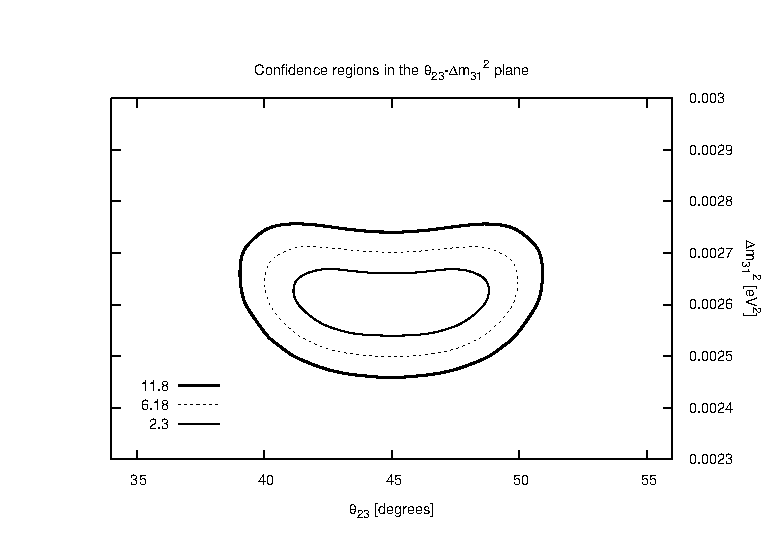
\includegraphics{T2K-2}
  \end{center}
  \vspace{-0.7 cm}
  \caption{Solution of problem 2. Confidence regions in the $\theta_{23}$--$\ldm$
    plane with the inclusion of spectral information.}
  \label{fig:th23dm31-spectral}
\end{figure}


\aufg{3}{The octant degeneracy}

Up to now, we have considered $\theta_{23}$ to be maximal. However, deviations
Of about $\pm 5^\circ$ from this best fit value are still compatible with
current data. Therefore, let us now consider the effect of $\theta_{23} = 40.0^\circ$.
Modify {\tt th23dm31.c} accordingly and compute the resulting confidence regions,
which should resemble Fig.~\ref{fig:th23dm31-nonmax}a. There are now two
distinct regions in the parameter space, which are both compatible with the
data at less than $1\sigma$: The correct one around $\theta_{23} = 40.0^\circ$,
and the degenerate one at $\theta_{23} = 90^\circ - 40.0^\circ$ (the so-called
octant degeneracy).

\begin{figure}
  \hspace{-0.7 cm}
  \begin{tabular}{cc}
    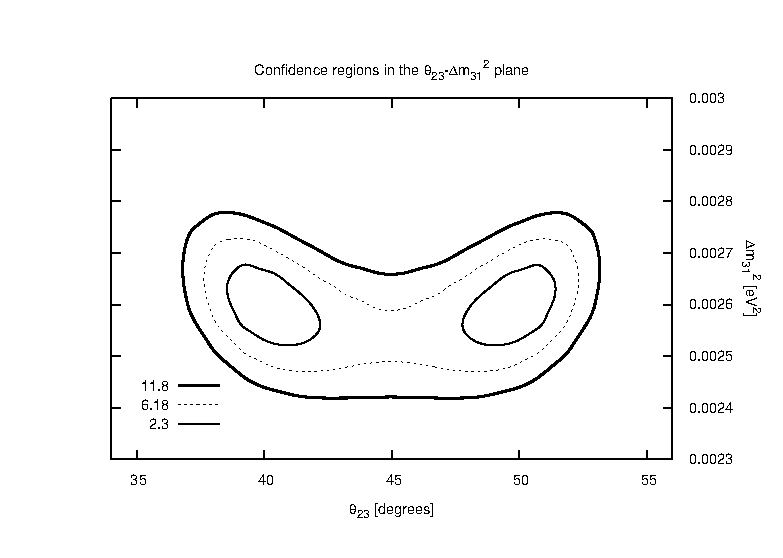
\includegraphics[width=8cm]{T2K-3}  & 
    \includegraphics[width=8cm]{T2K-4} \\
           (a)                   &          (b)
  \end{tabular}
  \caption{Solution of problem 3: Confidence regions in the $\theta_{23}$--$\ldm$
  plane for non-maximal $\theta_{23}$ and (a) zero $\theta_{13}$,
  (b) large $\theta_{13}$.}
  \label{fig:th23dm31-nonmax}
\end{figure}

This looks correct, but let us now increase $\theta_{13}$ to a value close
to the current upper bound, say, $\sthchooz = 0.1$. You will find that the
degenerate solution is now excluded at almost $2\sigma$ (Fig.~\ref{fig:th23dm31-nonmax}b).
Try to understand this feature from the (approximate) analytical expressions
for the neutrino oscillation probabilities:
\begin{align*}
  P_{\mu \mu} &= 1 - \sin^2 2\theta_{23} \, \sin^2 \Delta +
                    \alpha \, c_{12}^2 \, \sin^2 2\theta_{23} \, \Delta \, \sin 2\Delta \\
              & \ \ \ \ - \alpha^2 \, \Delta^2 \left[ \sin^2 2\theta_{12} \, c_{23}^2
                          + c_{12}^2 \, \sin^2 2\theta_{23} \left(\cos 2\Delta 
                          - s^2_{12} \right) \right]
                          + 4 \, s_{13}^2 \, s_{23}^2 \, \cos 2\theta_{23} \, \sin^2 \Delta \\
              & \ \ \ \ - 2 \, \alpha \, s_{13} \, \sin 2\theta_{12} \, s_{23}^2 \,
                                \sin 2\theta_{23} \, \cos \delta_{\rm CP} \, \Delta \, \sin 2\Delta\,,
    \\[3mm]
%
  P_{\mu e}^\mathrm{vac} &= \alpha^2 \, \sin^2 2\theta_{12} \, c_{23}^2 \, \Delta^2
                          + 4 \, s_{13}^2 \, s_{23}^2 \, \sin^2\Delta 
                          + 2 \, \alpha \, s_{13} \, \sin2\theta_{12} \sin2\theta_{23} \,
                              \cos(\Delta+\delta_{\rm CP}) \, \Delta \, \sin\Delta \,,
\end{align*}
where $\alpha = \sdm / \ldm$, $\Delta = \ldm L / 4E$, 
$s_{ij} = \sin\theta_{ij}$, and $c_{ij} = \cos\theta_{ij}$.


\aufg{4}{Incorporation of correlations with $\theta_{13}$ and $\delta_{CP}$}

Fig.~\ref{fig:th23dm31-nonmax}b should make us suspicious, since we do not
expect \TtoK\ to have the capability to resolve the octant degeneracy. Indeed,
we have so far assumed full knowledge about all oscillation parameters
except $\theta_{23}$ and $\delta_{CP}$, i.e.\ we have kept them fixed
at their ``true'' values in our fits. Unless there were some theoretical
argument (e.g.\ a flavor symmetry) pinning down these parameters, we
should allow them to vary within their presently allowed ranges in the fit.
This will yield smaller $\chi^2$ values, i.e.\ the sensitivity will decrease.

The marginalization over multi-dimensional subspaces of the oscillation
parameter space is one of the most powerful features of GLoBES.
To enable it in our code, we use the API functions {\tt glbAllocProjection},
{\tt glbDefineProjection}, {\tt glbSetDensityProjectionFlag}, and
{\tt glbSetProjection} to specify that $\theta_{12}$, $\theta_{13}$,
$\sdm$, and $\delta_{CP}$ should be marginalized over, while $\theta_{23}$,
$\ldm$, and the matter density should be kept at their initial values.
A short documentation of the required API functions is given in the
appendix.

Furthermore, we have to specify the parameters of the prior terms
\begin{align*}
  \chi^2_{\rm prior} = \frac{(x - x_0)^2}{\sigma_x^2},
\end{align*}
which can be added to $\chi^2$ for all oscillation parameters $x$ to
include external information on these parameters. Set all $x_0$ to the
{\tt true\_values} with the function {\tt glbSetCentralValues}, and use
{\tt glbAllocParams}, {\tt glbDefineParams}, {\tt glbSetDensityParams},
and {\tt glbSetInputErrors} to set
\begin{align*}
  \sigma_{\theta_{12}} &= 0.1 \cdot \theta_{12, \rm true} \\
  \sigma_\sdm          &= 0.1 \cdot \sdm_{\rm, true}.
\end{align*}
For all other parameters (including the matter density), we choose to omit
the prior terms by setting the respective $\sigma_x$ to 0.

Finally, we have to replace the call to {\tt glbChiSys} by one to {\tt glbChiNP}.
Due to the multi-dimensional minimization in the oscillation parameter space,
the calculation will now take a bit longer.\footnote{Note that our example
programs already use the faster, alternative minimization method GLB\_MIN\_POWELL
instead of the default GLB\_MIN\_NESTED\_POWELL. We emphasize, however, that
this is still an experimental feature in GLoBES 3.0.}
%For debugging, you
%can speed things up by switching off systematical errors with the command
%\begin{quote}
%  \ttfamily
%  glbSwitchSystematics(GLB\_ALL, GLB\_ALL, GLB\_OFF);
%\end{quote}
%This tells GLoBES to calculate $\chi^2$ according to the
%{\tt @sys\_off\_function} directives instead of the default
%{\tt @sys\_on\_function}. For \TtoK, this means using the $\chi^2$
%functions {\tt chiNoSysSpectrum} and {\tt chiNoSysTotalRates},
%which do not include any free systematical biases. In contrast to this,
%the default functions {\tt chiSpectrumTilt} and {\tt chiTotalRatesTilt}
%leave the normalization and tilt of the neutrino spectrum variable
%within the ranges defined by {\tt @signalerror} and {\tt @backgrounderror}.
%Thus, GLoBES has to fit these systematics parameters in addition to the
%oscillation parameters, which greatly increases the computational
%effort.

\begin{figure}
  \begin{center}
    \includegraphics{T2K-5}
  \end{center}
  \vspace{-0.7 cm}
  \caption{Solution of problem 4: Confidence regions in the $\theta_{23}$--$\ldm$
    plane for non-maximal $\theta_{23}$ and large $\theta_{13}$, including
    parameter correlations.}
  \label{fig:th23dm31-corr}
\end{figure}


\aufg{5}{The $\mathrm{sgn}(\ldm)$ degeneracy}

Besides the octant degeneracy, there is another degeneracy in the three-flavor
neutrino oscillation probabilities, which we have not considered ao far:
The ambiguity in the sign of $\ldm$. Indeed, if we considered the
half-plane of negative $\ldm$, we would find a mirror image of
Fig.~\ref{fig:th23dm31-corr}.

For the moment, however, we are only interested in the positions of the
two solutions with $\ldm < 0$. To find them, use the function {\tt glbChiAll},
and choose the starting values such that the minimizer will converge
to the appropriate local minima of $\chi^2$. Create a new {\tt glb\_params}
data structure and pass it to {\tt glbChiAll} as the second argument to
retrieve the position of the minimum.

Why is $|\ldm|$ slightly smaller at the degenerate solutions than at
the true one?



% ----------------------------------------------------------------------------
\section*{Part 2: Generic three-flavor effects: $\theta_{13}$ and $\delta_{CP}$}
% ----------------------------------------------------------------------------

\aufg{6}{Confidence regions in the $\theta_{13}$--$\delta_{CP}$ plane}

One of the main aims of superbeam experiments is the detection of
generic three-flavor effects, in particular of non-zero $\theta_{13}$
or $\delta_{CP}$. To examine the capability of \TtoK\ to measure these
parameters, we provide the program {\tt th13delta} and the accompanying
script {\tt th13delta.gnuplot}, which produces a confidence plot 
in the $\theta_{13}$--$\delta_{CP}$ plane. For simplicity, the program
only considers the normal mass hierarchy in the fit, i.e.\ we assume
that the $\mathrm{sgn}(\ldm)$ degeneracy has been resolved independently,
e.g.\ with supernova neutrinos. Furthermore, we have set the ``true''
$\theta_{23}$ back to $45^\circ$, so that we can also neglect the octant
degeneracy.

Fig.~\ref{fig:th13delta-orig} shows the results of the simulation.
As we can see from the plot, there is a strong correlation between
$\theta_{13}$ and $\delta_{CP}$, which makes it impossible to
efficiently constrain the CP phase. In the remainder of this
tutorial, we will consider two strategies for breaking this
correlation.

\begin{figure}
  \begin{center}
    \includegraphics{T2K-6}
  \end{center}
  \vspace{-0.7 cm}
  \caption{Output of {\tt th13delta}: Confidence regions in the
    $\theta_{13}$--$\delta_{CP}$ plane for a fit with the normal
    mass hierarchy.
    The ``true'' parameter values are $\theta_{23} = 45^\circ$,
    $\ldm = 2.6 \cdot 10^{-3}$~eV$^2$, $\sthchooz = 0.1$, and
    $\delta_{CP} = 90^\circ$.}
  \label{fig:th13delta-orig}
\end{figure}


\aufg{7}{Improving the sensitivity by anti-neutrino running}

One idea for improving the sensitivity of superbeam experiments is to operate
them in the anti-neutrino mode for several years after the neutrino running. 
Although the cross sections, and thus the event numbers, in the anti-neutrino
mode are smaller by a factor of three than those for neutrinos, one can
benefit from the fact that the dependence of the anti-neutrino oscillation
probabilities on $\delta_{CP}$ is different. To see the effect of this,
we need to incorporate a new flux definition, several new channels, and the
appropriate rules in th AEDL file. The parameters of these new AEDL
environments are mostly the same as for the existing ones, so you can start by
simply duplicating these. Give them new names, change the flux file to
{\tt JHFminus.dat}, and reverse the CP signs for the new channels.
Finnaly, increase the running time for the anti-neutrino mode to 6~years.

\begin{figure}
  \begin{center}
    \includegraphics{T2K-7}
  \end{center}
  \vspace{-0.7 cm}
  \caption{Solution of problem 7: Confidence regions in the
    $\theta_{13}$--$\delta_{CP}$ plane for 3~years of neutrino
    running, followed by 3~years of anti-neutrino running, and
    assuming the normal mass hierarchy.}
  \label{fig:th13delta-anti}
\end{figure}

As you can see from Fig.~\ref{fig:th13delta-anti}, the anti-neutrino running
will exclude almost half of the $\delta_{CP}$ values at the 90\% C.L., but
at $3\sigma$, the excluded region is much smaller.


\aufg{8}{Improving the sensitivity by incorporating reactor results}

Another option for breaking some of the correlations in \TtoK\ is the combination
with an advanced reactor neutrino experiment. To study this, incorporate
{\tt Reactor2.glb} into your simulation by adding an appropriate call to
{\tt glbInitExperiment}. Re-run the program to obtain
Fig.~\ref{fig:th13delta-reactor}, which shows that an advanced reactor
experiment can measure $\theta_{13}$ with a great precision. Moreover,
since the $\nu_e$ disappearance channel is independent of $\delta_{CP}$,
it does not suffer from parameter correlations. Therefore, the parameter
constraints that can be set by a combination of \TtoK\ and reactor data, are
competitive to those obtainable with the much more expensive anti-neutrino running.
Note, however, that this is only true as long is $\theta_{13}$ is
large. For smaller values, one cannot so easily benefit from reactor data.

\begin{figure}
  \begin{center}
    \includegraphics{T2K-8}
  \end{center}
  \vspace{-0.7 cm}
  \caption{Solution of problem 8: Confidence regions in the
    $\theta_{13}$--$\delta_{CP}$ plane for 3~years of \TtoK\ neutrino
    running, combined with {\tt Reactor2} data (exposure of
    8000~GW~kt~yrs), and assuming the normal mass hierarchy.}
  \label{fig:th13delta-reactor}
\end{figure}


% ----------------------------------------------------------------------------
\appendix
\section*{Appendix: Documentation of required API functions}
% ----------------------------------------------------------------------------

\begin{function}
{\tt glb\_params glbAllocParams()} allocates the memory space
needed for a parameter vector and returns a pointer to it.
\end{function}

\begin{function}
{\tt glb\_projection glbAllocProjection()} allocates the memory space
needed for a projection definition, and returns a pointer to it.
\end{function}

\begin{function}
{\tt double glbChiAll(const glb\_params in, glb\_params out, int exp)}
returns the minimized $\chi^2$ over all parameters for the experiment
{\tt exp}. For the simulation of all initialized experiments, use
{\tt GLB\_ALL} for {\tt exp}. The values in {\tt in} are the guessed
fit values for the minimizer. The actually determined parameters at
the minimum are returned in {\tt out}. If {\tt out} is set to {\tt NULL},
this information will not be returned.
\end{function}

\begin{function}
{\tt double glbChiNP(const glb\_params in, glb\_params out, int exp)}
returns the projected $\chi^2$ onto the hyperplane specified by
{\tt glbSetProjection} for the  experiment {\tt exp}.
For the simulation of all initialized experiments,
use {\tt GLB\_ALL} for {\tt exp}. The values in {\tt in} are the guessed
fit values for the minimizer (all free parameters) and the fit values
on the hyperplane (all fixed parameters). The actually determined parameters
at the minimum are returned in {\tt out}, where the fixed parameters are
still at their input values. If {\tt out} is set to {\tt NULL}, this
information will not be returned.
\end{function}

\begin{function}
{\tt glb\_params glbDefineParams(glb\_params in, double theta12, double
theta13, \\ double theta23, double delta, double dms, double dma)}
assigns a set of oscillation parameters to the vector {\tt in}, which
has to be allocated before. The return value is the pointer to {\tt in}
if the assignment was successful, and {\tt NULL} otherwise.
\end{function}

\begin{function}
{\tt glb\_projection glbDefineProjection(glb\_projection in, int theta12,
int \\ theta13,int theta23, int delta, int dm21, int dm31)} defines a
projection in the oscillation parameter space. For each parameter,
the function expects one of the flags {\tt GLB\_FREE} or {\tt GLB\_FIXED},
indicating whether the respective parameter is to me marginalized over
or not. The return value is the pointer to {\tt in} if
the assignment was successful, and {\tt NULL} otherwise.
\end{function}

\begin{function}
{\tt void glbFreeParams(glb\_params stale)} frees the memory
needed for a parameter vector {\tt stale}.
\end{function}

\begin{function}
{\tt void glbFreeProjection(glb\_projection stale)} frees the memory
needed for the projection definition vector {\tt stale}.
\end{function}

\begin{function}
{\tt int glbInitExperiment(char *inf, glb\_exp *in, int *counter)}
adds a single experiment with the filename {\tt inf} to the list of currently
loaded experiments. The {\tt counter} is a pointer to the variable containing
the number of experiments (normally {\tt \&glb\_num\_of\_exps}), and
{\tt in} points to the beginning of the experiment list (normally
{\tt \&glb\_experiment\_list[0]}). The function returns zero if it was
successful.
\end{function}

\begin{function}
{\tt int glbSetCentralValues(const glb\_params in)} sets the central
values for the prior terms to {\tt in}.
\end{function}

\begin{function}
{\tt glb\_params glbSetDensityParams(glb\_params in, double dens, int which)}
sets the density parameter for experiment number {\tt which} in the structure
{\tt in} to the value {\tt dens}. If the assignment was unsuccessful, the
function returns {\tt NULL}. If {\tt GLB\_ALL} is used for {\tt which},
the density parameters of all experiments will be set.
\end{function}

\begin{function}
{\tt glb\_projection glbSetDensityProjectionFlag(glb\_projection in,
int flag, int which)} specifies whether the matter density in experiment
number {\tt which} should be marginalized over ({\tt flag} = {\tt GLB\_FREE})
or not ({\tt flag} = {\tt GLB\_FIXED}). The return value is the pointer to {\tt in}
if the assignment was successful, and {\tt NULL} otherwise.
\end{function}

\begin{function}
{\tt int glbSetInputErrors(const glb\_params in)}
sets the input errors for all of the following minimizer calls to {\tt in}.
An input error of $0$ corresponds to not taking into account the
respective prior.
\end{function}

\begin{function}
{\tt int glbSetProjection(const glb\_projection in)} sets the projection
to {\tt in}. The return value is $0$ if successful, and $-1$ if
unsuccessful.
\end{function}


\end{document}


